\paragraph{}
Due to the fact that there are a few error indicators, it could be hard to determine the relationship between them and whether a subdomain needs refinement or not.
As a result, specific technique is required in order to search for the patterns in the data to find this relationship.
After that, the final decision which is a binary classification in this case as each subdomain will be labeled as ``refine'' or ``not refine'' can be made based on the input of the error indicators explained in Sec.~\ref{adap_sec:error_indicator}.
Hence, the discovery of regularities plays a key role in the adaptive analysis and an automatic discovery of regularities is usually associated with pattern recognition by the help of algorithms.

%   ----    %
\subsection{Training Set}
\paragraph{}
The training set is determined by numerical examples in Fig.~\ref{adap_fig:svm_train_chole} and Fig.~\ref{adap_fig:svm_train_cantilever}.
The training data is annotated with whether a subdomain is refined or not and the model can study the data and learn to classify each subdomain based on all four features explained in \ref{adap_sec:error_indicator}.
\begin{figure}[!ht]
    \centering
    \begin{subfigure}[b]{0.5\linewidth}
        \scalebox{0.5}{
            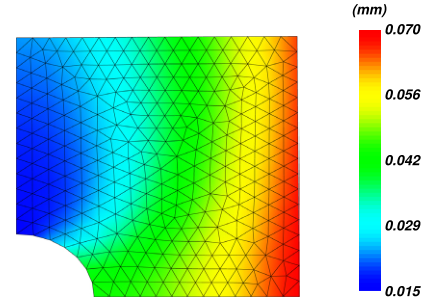
\includegraphics{adaptivity/images/adap_svm_train_chole_0.png}
        }
        \caption{Mesh and displacement field before refinement}
    \end{subfigure}
    \begin{subfigure}[b]{0.5\linewidth}
        \scalebox{0.45}{
            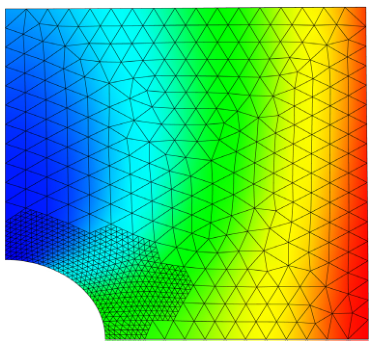
\includegraphics{adaptivity/images/adap_svm_train_chole_1.png}
        }
        \caption{Mesh and displacement field after refinement}
    \end{subfigure}
    \caption{Mesh refinement for square plate with circular hole \citep{Duval2018}}
    \label{adap_fig:svm_train_chole}
\end{figure}

\begin{figure}[!ht]
    \centering
    \begin{subfigure}[b]{0.4\linewidth}
        \scalebox{0.6}{
            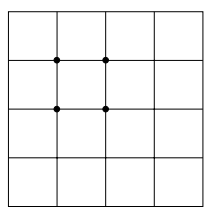
\includegraphics{adaptivity/images/adap_svm_train_cantilever_0.png}
        }
    \end{subfigure}
    \begin{subfigure}[b]{0.4\linewidth}
        \scalebox{0.6}{
            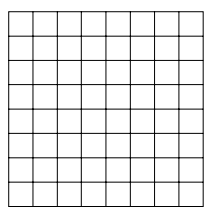
\includegraphics{adaptivity/images/adap_svm_train_cantilever_1.png}
        }
    \end{subfigure}\\
    \begin{subfigure}[b]{1\linewidth}
        \centering
        \scalebox{0.7}{
            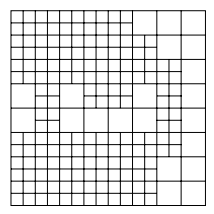
\includegraphics{adaptivity/images/adap_svm_train_cantilever_2.png}
        }
    \end{subfigure}
    \caption{Mesh refinement of a short cantilever beam \citep{Zienkiewicz2005500}}
    \label{adap_fig:svm_train_cantilever}    
\end{figure}
%
With the same examples, uniform mesh of quadtree is conducted and the same region are marked as refined as shown in Fig.~\ref{adap_fig:svm_train_my}.
\begin{figure}[!ht]
    \centering
    \begin{subfigure}[b]{1\linewidth}
        \centering
        \scalebox{0.25}{
            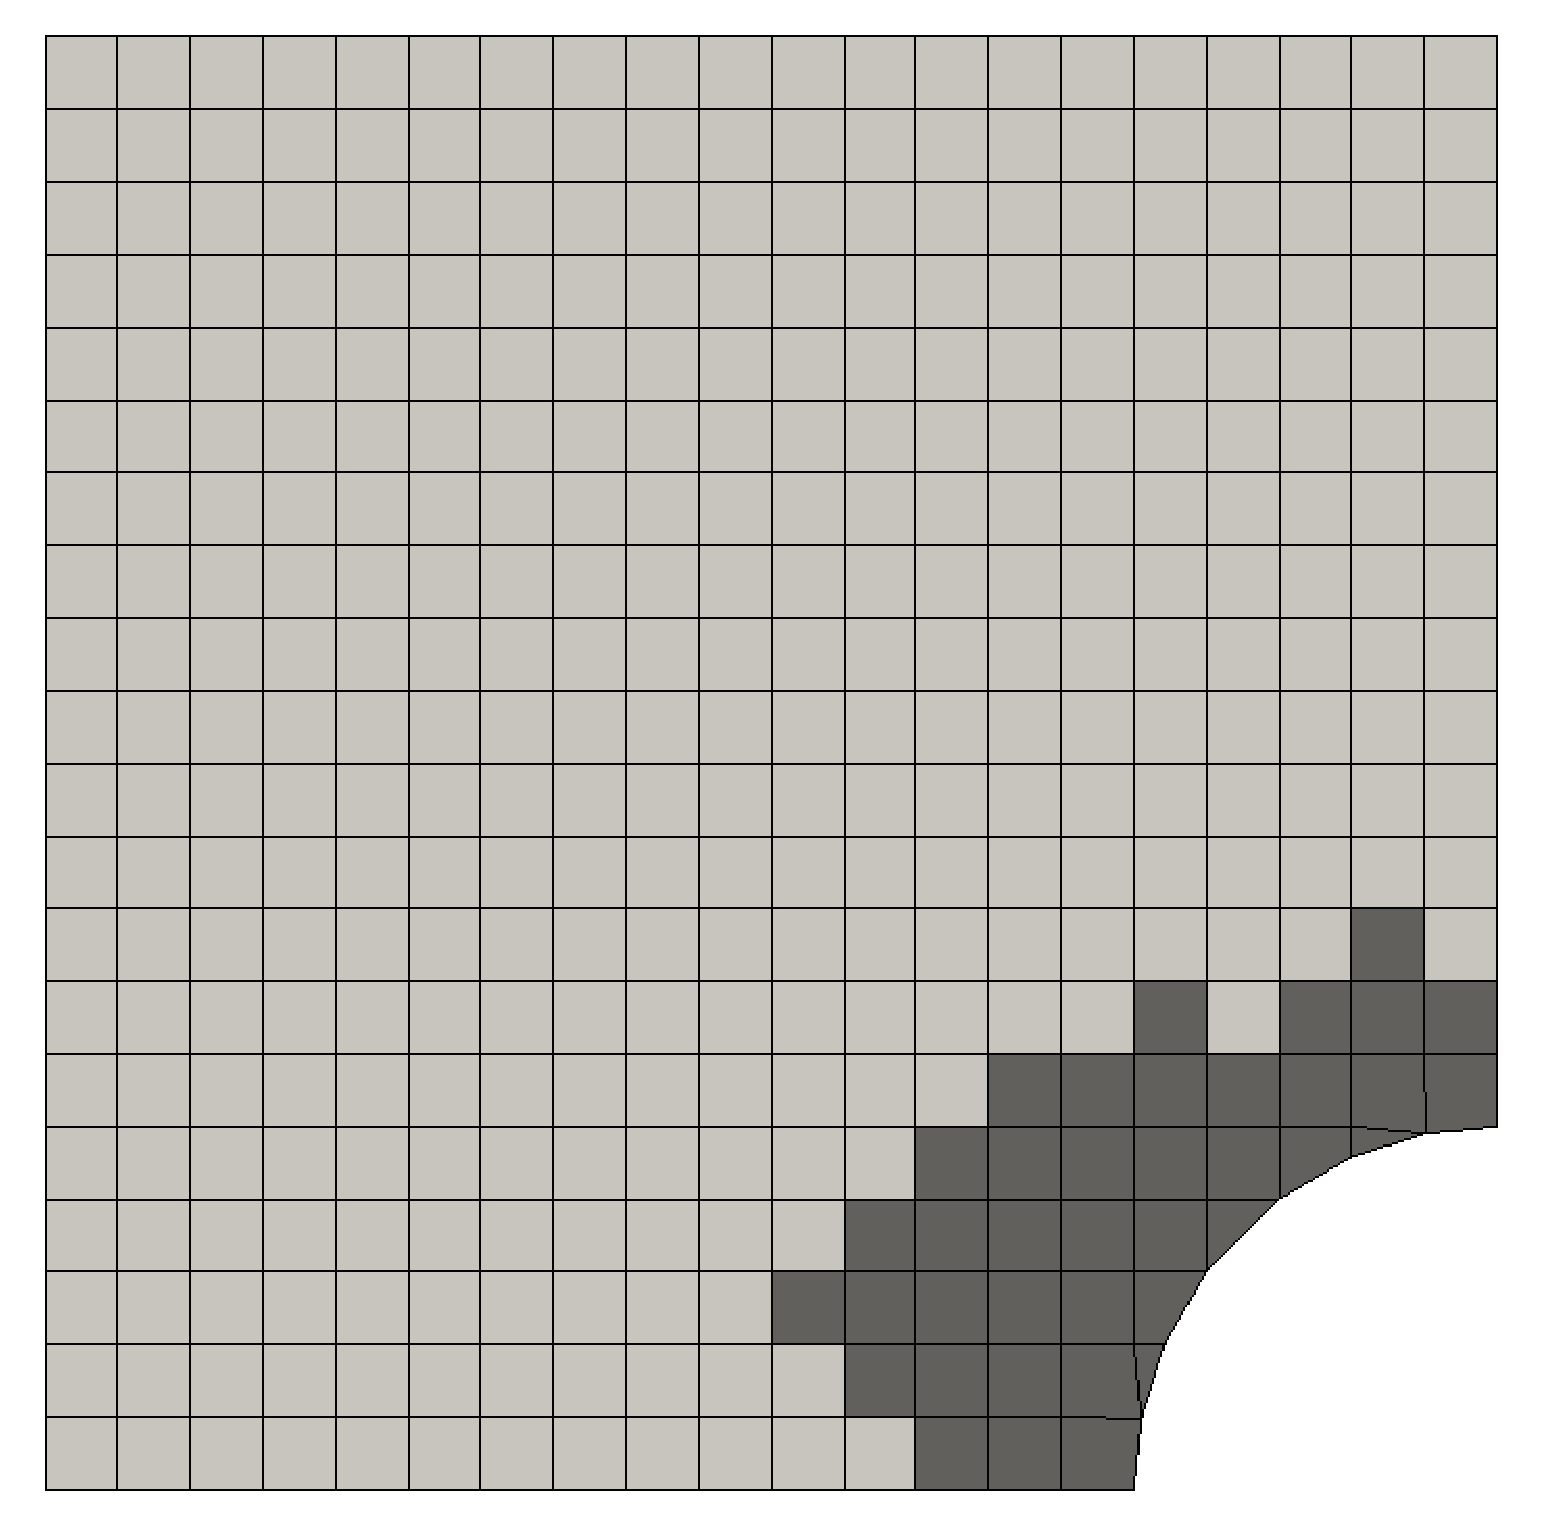
\includegraphics{adaptivity/images/adap_svm_train_my_chole.eps}
        }
    \end{subfigure}
    \begin{subfigure}[b]{0.49\linewidth}
        \scalebox{0.25}{
            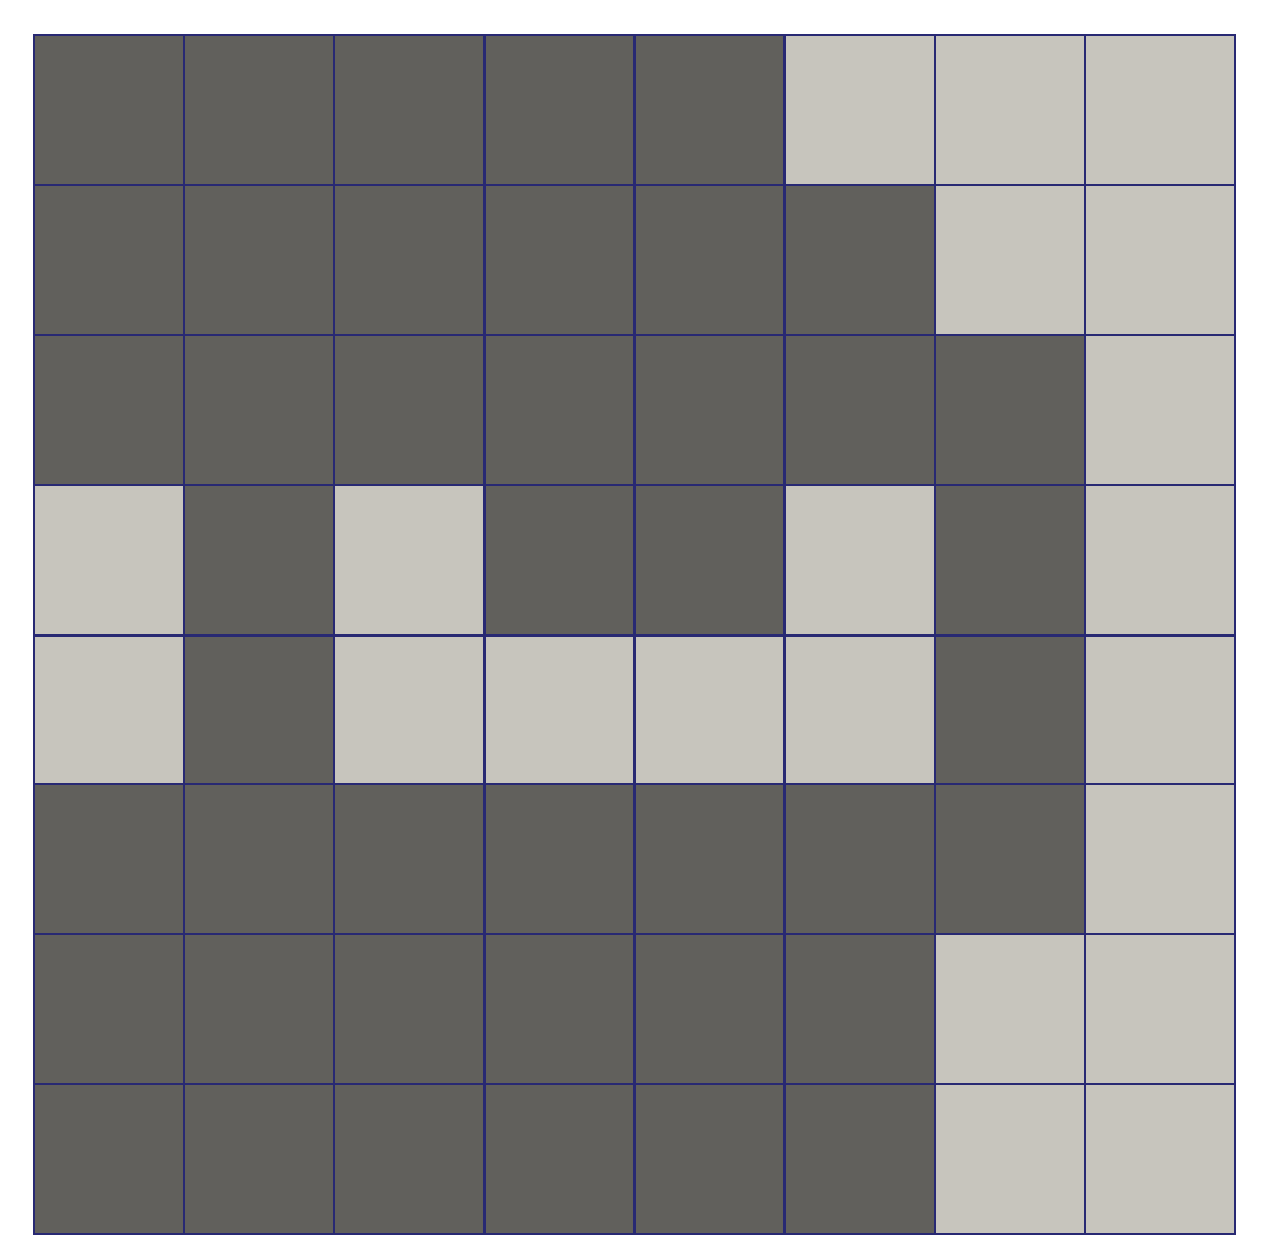
\includegraphics{adaptivity/images/adap_svm_train_my_cantilever_0.eps}
        }
    \end{subfigure}
    \begin{subfigure}[b]{0.49\linewidth}
        \scalebox{0.25}{
            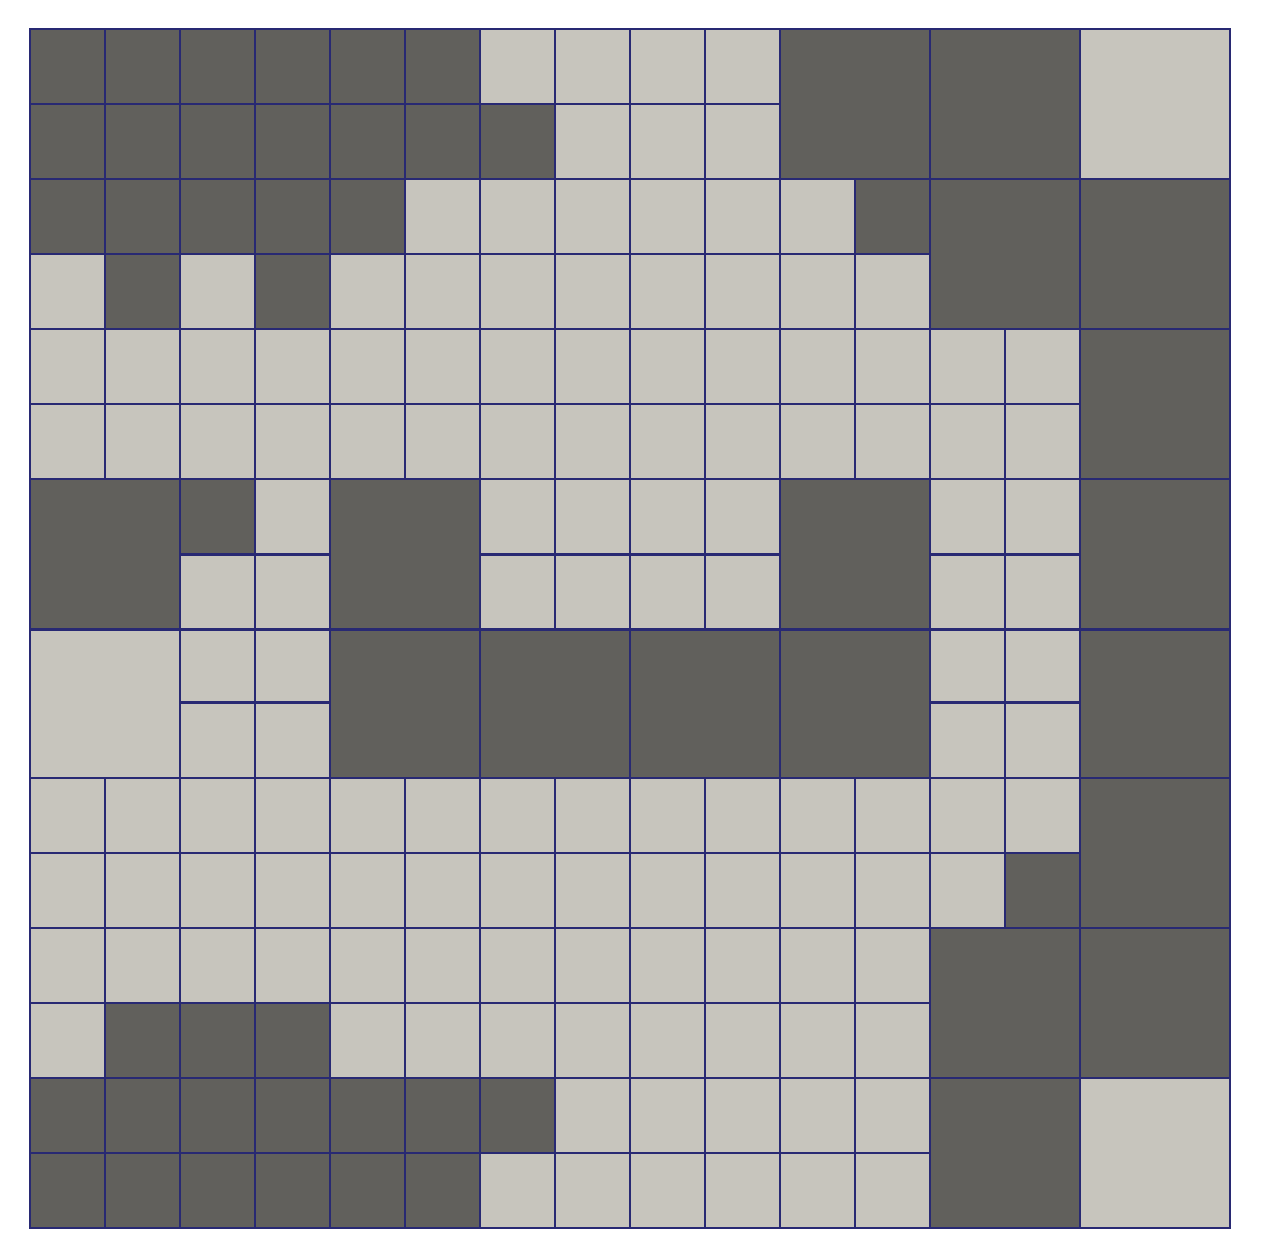
\includegraphics{adaptivity/images/adap_svm_train_my_cantilever_1.eps}
        }
    \end{subfigure}
    \caption[Training data for SVM]{Training data for SVM: Cells in black is marked as refined.}
    \label{adap_fig:svm_train_my}
\end{figure}
%
Criteria taken into consideration are: 
\begin{enumerate}
    \item Ratio of the area of the cell to the total area
    \item Minimal angle formed by the intersecting lines connected by scaling center and adjacent polygon vertexes
    \item Eigenvalue error indicator for displacement
    \item Eigenvalue error indicator for stress
\end{enumerate}
%
\subsection{Regularization for MLP}
\paragraph{Bagging}
\label{adp_sec:ml_bagging}
Bagging is a technique that utilize multiple models in order to increase the accuracy of the prediction \citep{Breiman1996}.
The principle of idea of that is simple: training multiple models separately and let them vote for the prediction.
It is adopted vastly in machine learning.
The idea behind the optimization technique is that different models often make different errors on the same test set.
Take a set of $k$ regression models for an example, error $\epsilon_i$ is made by each model on each example.
The errors are drawn from a zero-mean multivariate normal distribution with variances $E[\epsilon_i^2]$ = $\nu$ and covariances $E[\epsilon_i \epsilon_j]$=$c$.
As a result, the overall error determined by averaging of all models is $\frac{1}{k}\sum_i \epsilon_i$.
The expected squared error of the ensemble predictor is
\begin{equation}
    \begin{aligned}
    E[(\frac{1}{k} \sum_i \epsilon)^2] &=
    \frac{1}{k^2}[
        \sum_i (
            \epsilon_i^2 + \sum_{j\neq i}\epsilon_i \epsilon_j
        )
    ] \\
    &= \frac{1}{k}\nu + \frac{k-1}{k}c
    \end{aligned}
\end{equation}
%
The bagging technique does not help if the errors are highly correlated and $c=\nu$ as the mean squared error can reduce to $\nu$.
On the other hand, the effect of this technique may be significant if the errors are highly uncorrelated and $c=0$, in which situation the overall mean squared error becomes $\frac{1}{k}\nu$.
In other words, the overall mean squared error decreases linearly with the model size.
To conclude, the performance of this technique must not be worse than any of its individual model and a significant improvement can be expected if its members make independent errors.

\paragraph{}
There are several different methods to train ensemble.
For instance, each member of the ensemble can be trained with same training set but different algorithms or different training set with same algorithm.
The reuse of the same kind of models and algorithms is allowed thanks to the bagging.
The bagging technique used in the proposed method is constructing $k$ different training set.
Each training is built by sampling the original data set randomly.
In other words, each individual model may have some dataset which is not appear in any other models.
There is also some dataset are shared by multiple models.

\paragraph{}
Due to the large number of initialization parameter for a neural network, bagging technique can be extremely effective because the random selection of parameters such as initialized weight, mini-batches, hyper-parameters and so on leads to a different outcome even with the same training data.
The method is proved to be reliable and powerful for minimizing the generalization error.
Averaging dozens of models is widely adopted in those who won the machine learning contests and a recent example is Netflix Grand Price \citep{koren2009}.


\paragraph{Dropout}
Dropout \citep{JMLR:v15:srivastava14a} is another optimization approach used in the proposed method.
An effective but computationally cheap regularizing technique is provided.
Roughly speaking, the dropout can be regarded as one method to create different models in bagging described in Sec.~\ref{adp_sec:ml_bagging} by training multiple models.
One problem in bagging is that it could be impractical when each model is so large that the training can be computationally expensive in terms of time and space complexity.
Hence, the number of models used in ensembles tends to be in the range of $5$ and $10$ and the winner of ILSVRC \citep{DBLP:journals/corr/SzegedyLJSRAEVR14} used $6$ models.
As a comparison, dropout provides an cheap algorithm that can train and evaluate a large number of bagged ensemble.

\paragraph{}
In dropout, random hidden units are disabled during the training, which can be easily achieved by manually setting the weight to zero.
By doing so, the contribution of this hidden unit is ignored based on the fact that matrix production is used.
It can also be implemented by removing the unit completely from the network.
In bagging technique, $k$ different models with different training data are trained.
This is shared by the dropout as well, while dropout supports larger number of neural networks.
During the training process using dropout, a minibatch-based learning algorithm introduced in Sec.~\ref{lr_sec:ml_sgd} is used to make insignificant steps.
Whenever a sample is loaded into the minibatch, a random binary mask is applied to all of the inputs and hidden units in the network.
The probability a unit be disabled is independent from others and shall be determined from the user input as one of the hyperparameter.
In the proposed method, an input units has $20\%$ chance of being disabled and the number is $50\%$ for the hidden units.


\paragraph{}
More formally, assume that a mask vector $\mu$ specifies which units to include and $J(\theta,\mu)$ defines the cost of the model defined by parameters $\theta$ and mask $\mu$ \citep{Goodfellow-et-al-2016}.
After that, the training of the dropout becomes minimizing $E_\nu J(\theta,\mu)$.
The expectation may includes great number of terms while it could be possible to determine an unbiased estimation of its gradient by sampling values of $\mu$.

\paragraph{}
The training of the dropout is quite different to that of bagging.
Models use same parameters but different training data in bagging as shared parameters help to represent numerous number of models without occupying too many memory.
During the training using bagging, individual model is trained until convergence while during the training using dropout, most of the models are not explicitly trained.
That is because the number of the possible sub-network in dropout is too significant to finish the training within the lifetime of the universe.
Instead, only minor proportion are trained for a single step.
Parameter sharing guarantee that the remaining sub-networks are able to arrive at good settings.
The bagging algorithms are followed after that.
For instance, the training data used by individual model actually is sampled from the original training set.
Simple majority of the votes from all members are adopted to determine the prediction of the ensemble.
Although bagging and dropout does not require a explicitly probabilistic model, it is assumed that a probability distribution $p^{(i)}(y|x)$ will be the output.
The prediction of the ensemble is given by averaging all these distributions,
\begin{equation}
    \frac{1}{k} \sum_{i=1}^k (y|x)
\end{equation}
%
For dropout, individual model with a mask vector $\mu$ defines a probability distribution $p(y|x, \mu)$.
The arithmetic mean over all masks is given by
\begin{equation}
    \sum_\mu p(\mu) p(y|x, \mu)
    \label{adap_eq:ml_dropout_sum}
\end{equation}
%
where $p(\mu)$ is the probability distribution used to sample $\mu$ during the training.
Since numerous number of terms are involved in the summation, it could be difficult to calculate Eq.~\ref{adap_eq:ml_dropout_sum} without simplification.
However, a deep neural network do not allow such simplification.
Instead, it is possible to approximate the simplification with sampling by calculate the mean value from many masks.
It is suggested that around $15$ masks are able to provide satisfactory performance \citep{Goodfellow-et-al-2016}

\paragraph{}
Yet, the existence of a better approach allows the determination of a satisfactory approximation to the predictions of the ensemble at the cost of one forward propagation.
It can be achieved by adopting geometric mean instead of the arithmetic mean of the ensemble member's predicted distributions \citep{WardeFarley2014SelfinformedNN}.
However, using the geometric mean instead of the arithmetic mean leads to the result which is not guaranteed to be a probability distribution.
In order to enforce a probability distribution as the result, the requirement that all sub-models must assign a non-zero probability to all events is imposed.
After that, the resulted distribution is normalized again.
The unnormalized probability distribution from geometric mean is:
\begin{equation}
    \tilde{p}_{ensemble}(y|x) = 2^d \sqrt{\prod_\mu p(y|x,\mu)}
\end{equation}
%
where $d$ is the number of units that my be dropped.
To simplify the presentation, a uniform distribution over $\mu$ is adopted.
But it should be noted that non-uniform distributions can be treated as well.
Eq.~\ref{adap_eq:ml_renormalize} need to be performed on the ensemble in order to determine the prediction
\begin{equation}
    p_{ensemble}(y|x) = \frac{
        \tilde{p}_{ensemble}(y|x)
    }{
        \sum_{y^\prime} \tilde{p}_{ensemble}(y^\prime|x)
    }
    \label{adap_eq:ml_renormalize}
\end{equation}
%
The key idea behind the dropout is to approximate $p_{ensemble}$ by calculating $p(y|x)$ in one model \citep{hinton2012}.
The aim of this improvement is to capture the correct output from that unit.
It is called weight scaling inference rule which shows outstanding performance empirically.
\paragraph{}
Since an inclusion probability of $\frac{1}{2}$ is widely adopted, the weight scaling rule tends to half the weights after training.
The model is used as usual after that.
It can also be achieved by multiplying the states of the units by $2$ during training.
Both of these two methods are to narrow the difference between the expected total input to a unit at test time and that at the training when approximately half of the hidden units are dropped.
For those models without nonlinear hidden units, the weight scaling inference rule gives exact result.
For instance, a softmax regression classifier with $n$ input variables represented by the vector $v$ is considered:
\begin{equation}
    P(y=y|v)=softmax(W^Tv+b)_y
\end{equation}
%
They can be indexed into the family of sub-models by element-wise multiplication of the input with a binary vector $d$:
\begin{equation}
    P(y=y|v;d) = softmax(W^T(d \odot v)+b)_y
\end{equation}


\subsubsection{Indicator used in adaptivity}
\paragraph{}
All terms used in the performance indicators in machine learning are introduced in Sec.~\ref{lr_ml:indicators}
The balance of the indicators is highly dependent on classifiers' objective.
Take the spam detector for an example, a false positive can be more dangerous than a false negative as an important e-mail being marked as spam can be a disaster.
While in adaptivity, there may be no favour over either of them.
It is because the refinement of a cell with lower error or leaving a cell with higher error unrefined may not produce significant influence on the final result.
As a result, F1 score can be the most important indicator as it takes both recall rate and precision into consideration.


\subsection{Result}
\paragraph{}
All training data are standardized by Eq.~\ref{adap_eq:svm_standardized} where $\overline{x}$ and $\sigma$ is the mean and standard deviation of the data.
It makes features in training data have zero means and unit variance.
Cells that need to be refined are labeled as $1$ and the rest are labeled as $0$.
Radial basis function with $\sigma=0.7624$ is adopted as kernel function in SVM.
    \begin{equation}
        x^\prime = \frac{x-\overline{x}}{\sigma}
        \label{adap_eq:svm_standardized}
    \end{equation}
Half of the training data ($320$ out of $640$) are used to train the model and the reset are used for cross validation.
Different class weights are set for testing different performance in regard to all indicators in Fig.~\ref{adap_fig:svm_performance_0}.
\begin{figure}[h!]
    \centering
    \scalebox{0.3}{
        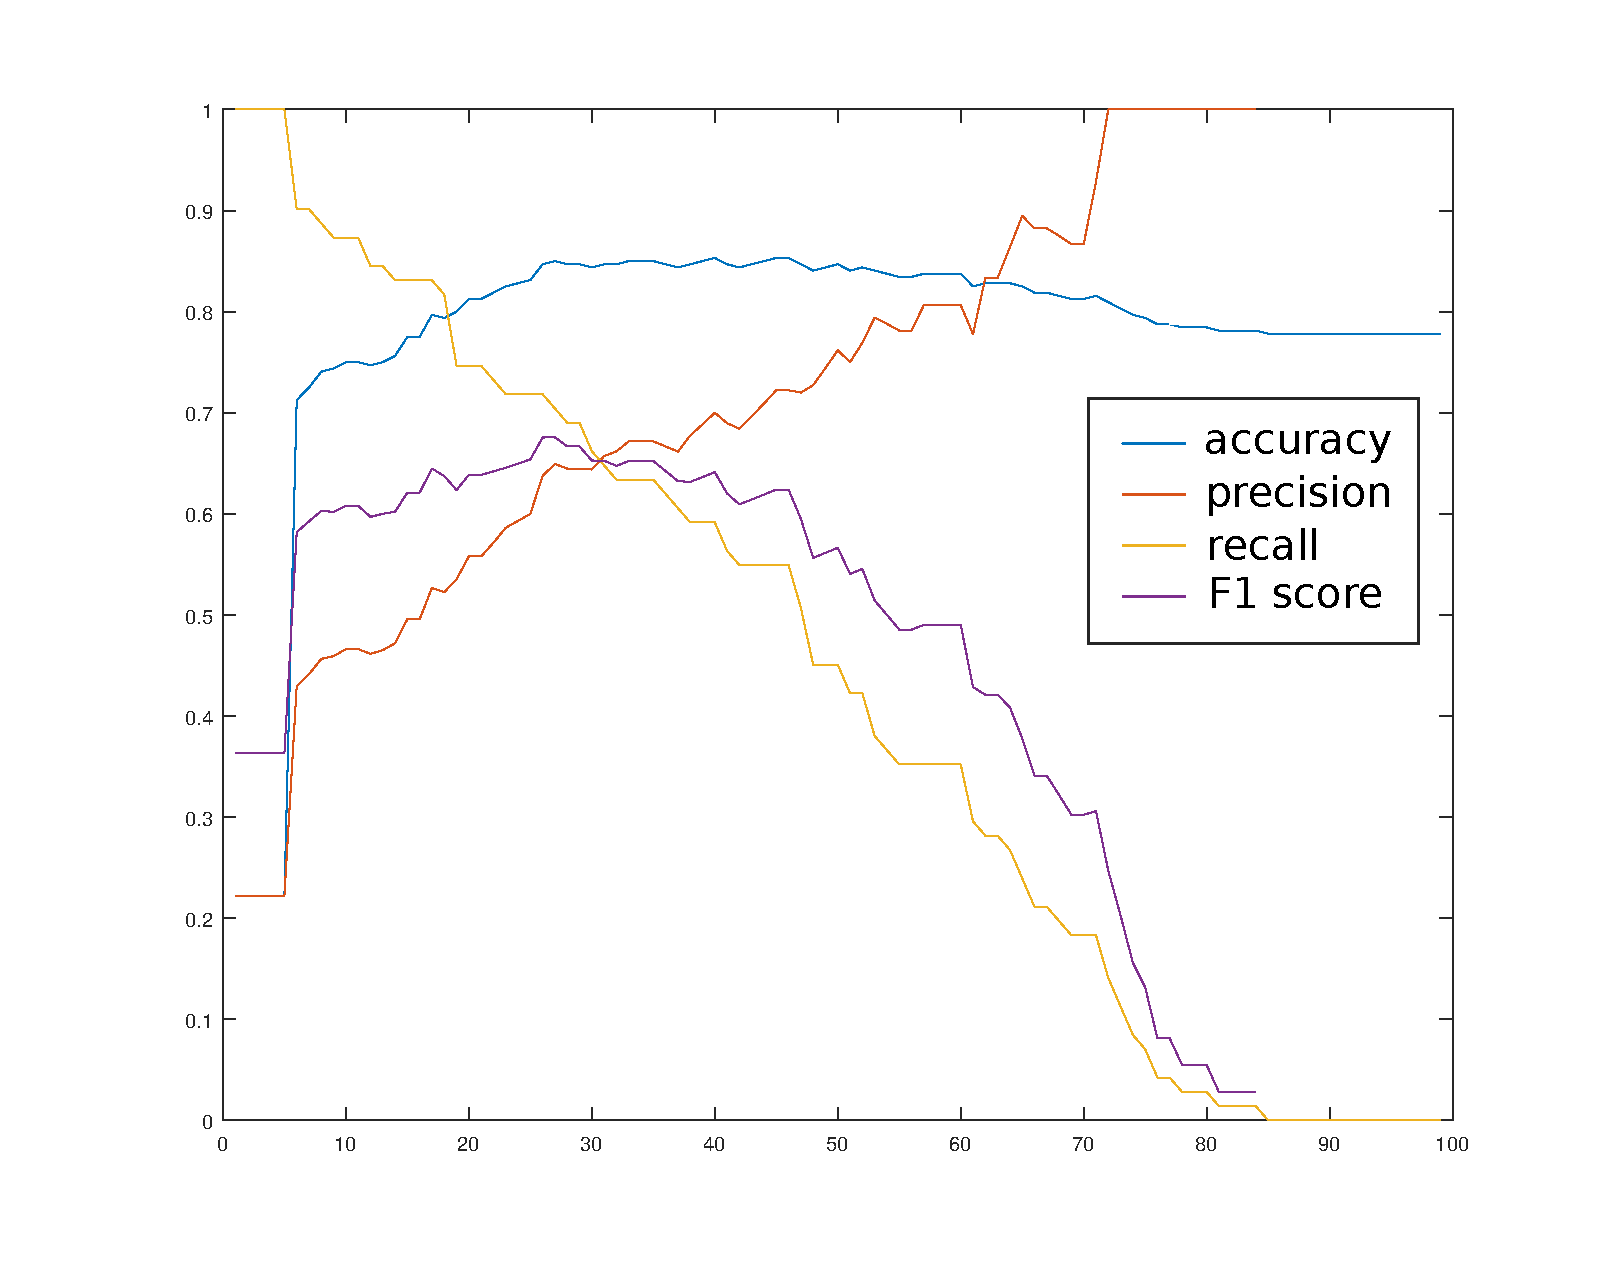
\includegraphics{adaptivity/images/svm_performance_0.eps}
    }
    \caption{Accuracy, precision, recall rate and F1 score vs different class weight}
    \label{adap_fig:svm_performance_0}
\end{figure}
%
A class weight is a vector that influence the predication directly.
The model will calculate the probability for each classification based on the input and the one with higher probability will be chosen as the result in default situation.
Change class weight to $1:2$ will force the model to choose first class when its probability is higher than $66.67\%$ instead of $50\%$.
A class weight of $3:7$ was chosen from Fig.~\ref{adap_fig:svm_performance_0} to guarantee a balance between precision and recall rate.
The corresponding result is listed in Tab.~\ref{adap_tab:svm_result}.
\begin{table}[h!]
    \centering
    \caption{Result of cross validation}
    \begin{tabular}{cc}
        \toprule
        Accuracy    &   84.38\%    \\
        Precision   &   64.38\%     \\
        Recall rate &   66.20\%     \\
        F1 score    &   65.28\%     \\
        \bottomrule
    \end{tabular}
    \label{adap_tab:svm_result}
\end{table}
%  compare auc
\pagebreak